%------------------------------------------------------------------------------
% Author(s):
% Varaun Ramgoolie
%
% Copyright:
%  Copyright (C) 2020 Brad Bachu, Arjun Mohammed, Varaun Ramgoolie, Nicholas Sammy
%
%  This file is part of Applied-Mathematics-Unit2 and is distributed under the
%  terms of the MIT License. See the LICENSE file for details.
%
%  Description:
%     Year: 2008 May
%     Module: 3
%     Question: 6
%------------------------------------------------------------------------------

%------------------------------------------------------------------------------
% 6 a
%------------------------------------------------------------------------------

\begin{subquestions}
	
\subquestion

\begin{subsubquestions}
	
\subsubquestion

Newton's Second Law states that, the rate of change of linear momentum of an object is directly proportional to the Resultant Force which acts on the object. We can represent this mathematically as,
\begin{align} 
	\text{Resultant Force} & \propto \ddd{\vec{p}}{t} \nn \\
	             & \propto \frac{\Delta \vec{p}}{\Delta t} \nn \\
	             & \propto \frac{m\vec{v}-m\vec{u}}{\Delta t} \nn \\
	             & \propto m\frac{\vec{v}-\vec{u}}{\Delta t} \nn \\
	             & = m\vec{a} \,.
\end{align}

It should be noted that $\vec{F}$ and $\vec{a}$ are vector quantities. \footnote{This means that the equality holds in their respective directions.}
\end{subsubquestions}
	
%------------------------------------------------------------------------------

\subsubquestion
	
\textbf{\textit{Sketch and Translate:}} \\ \\
It is given that a particle is thrown up in the air with an initial speed, $u$ and varying resistive forces act against it.
See \rfig{2008M:q6:Sketch1}.
\begin{figure}[H]
	\begin{center}
		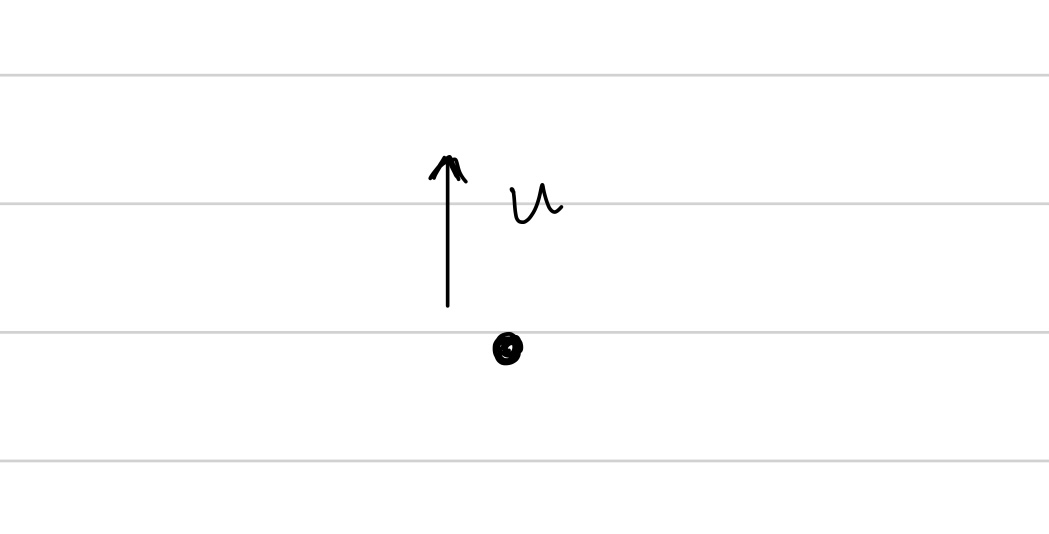
\includegraphics[scale=0.25]{../2007/figures/2008Mq6Sketch}
		\caption{\label{2008M:q6:Sketch1} Particle at launch.}
	\end{center}
\end{figure}




\textbf{\textit{Simplify and Diagram:}} \\ \\
\rfig{2008M:q6:Diagram1} shows all of the forces acting on the particle.
\begin{figure}[H]
	\begin{center}
		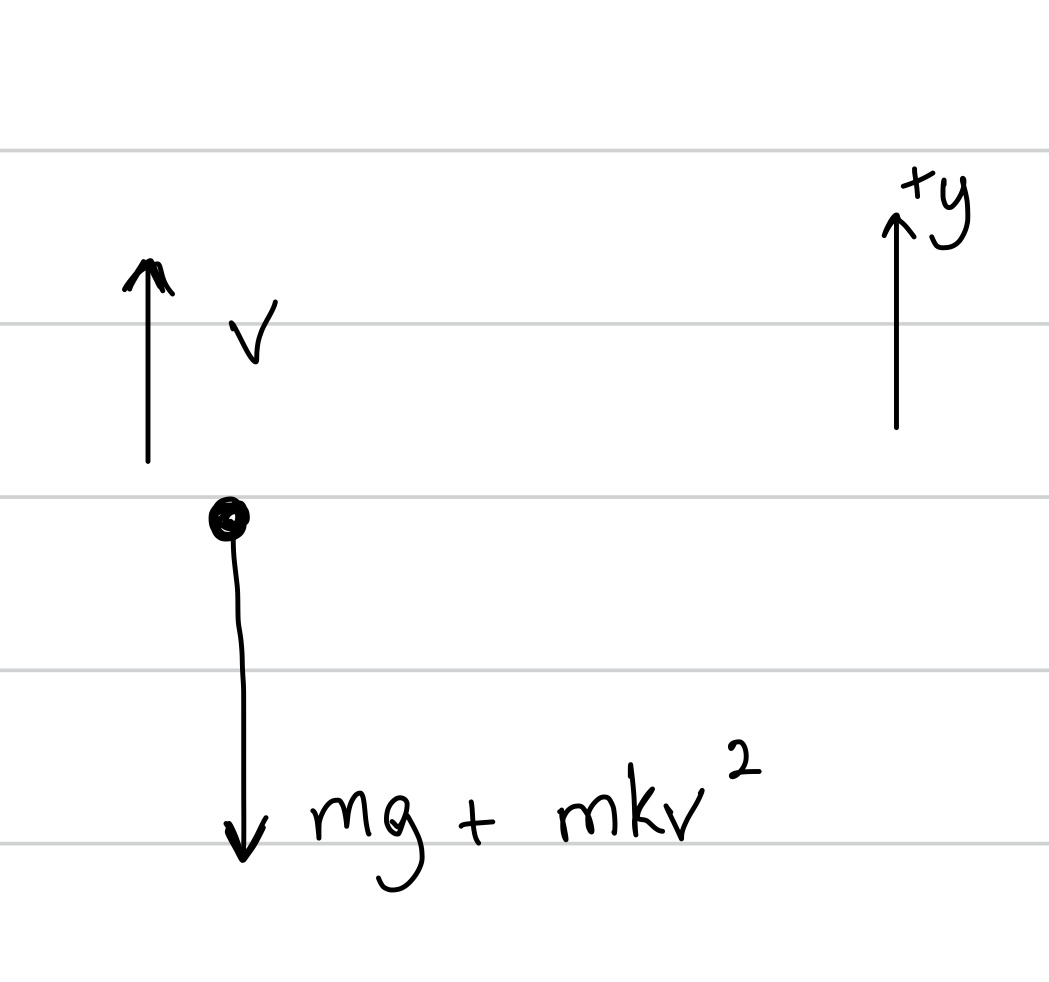
\includegraphics[scale=0.25]{../2007/figures/2008Mq6Diagram}
		\caption{\label{2008M:q6:Diagram1} Free body diagram of the particle.}
	\end{center}
\end{figure}

We want to find an expression for the greatest height reached by the particle. From Newton's 2nd Law, we know that the particle must have an acceleration in the $-y$ direction. Since we know that the resultant force (and by extension, the acceleration) is dependent on the speed of the particle, $v$, in the $+y$ direction, we can formulate an expression for the height of the particle and solve for the greatest height.

We should notice that, at the greatest height $y_{\text{max}}$, the velocity of the body, $v$, must be 0 as it is the point where it changes direction from upwards motion to downwards motion.
We will represent the movement of the particle in the $y$ direction as $s_y$.
We should also assume that no other forces act on the particle except for those in \rfig{2008M:q6:Diagram1}. 




\textbf{\textit{Represent Mathematically:}} \\ \\
As there are no forces in the $x$ direction, we only need to consider the $y$ direction. From Newton's Second Law, we see that,
\begin{align}
	\sum \vec{F} & = m\vec{a} \nn \\
	-(mg+mkv^2) \yhat & = ma \yhat \nn \\
	\implies a \yhat & = (-g -kv^2)\yhat \,.
\end{align}

As we can see, the acceleration in the $y$ direction is dependent on $v^2$. We can formulate a differential equation as follows,
\begin{align}
	a & = -g -kv^2 \nn \\
	v \ddd{v}{s_y} & = -g - kv^2 \nn \\
\end{align}

Separating these variables, we get,
\begin{align}
	\dd s_y & = \frac{-v}{g+kv^2}\dd v \nn \\
	\int_{y_1}^{y_2} \dd s_y & = \int_{v_1}^{v_2} \frac{-v}{g+kv^2}\dd v \,.
\end{align}




\textbf{\textit{Solve and Evaluate:}} \\ \\
From our given information, we know that when $s_y=0$, $v=u$, and when $s_y=y_{\text{max}}$, $v=0$. Using these as our bounds of integration, we get that,
\begin{align}
	\int_{0}^{y_{\text{max}}} \dd s_y & = \int_{u}^{0} \frac{-v}{g+kv^2}\dd v \nn \\
	\int_{0}^{y_{\text{max}}} \dd s_y & = \frac{-1}{2k}\int_{u}^{0} \frac{2kv}{g+kv^2}\dd v \nn \\
	\left[s_y\right]_0^{y_{\text{max}}} & = \frac{-1}{2k} \left[\ln(g+kv^2)\right]_u^0 \nn \\
	y_{\text{max}} & = \frac{-1}{2k} \left[\ln(g)-\ln(g+ku^2)\right] \nn \\
	               & = \frac{1}{2k} \left[\ln(g+ku^2)-\ln(g)\right] \nn \\
	               & = \frac{1}{2k} \left(\ln\left(\frac{g+ku^2}{g}\right)\right) \nn \\
	 			   & = \frac{1}{2k} \left(\ln\left(1 + \frac{ku^2}{g}\right)\right) \,.
\end{align} \footnote{In our second line, we use a trick to integrate this function. By multiplying by $\frac{2k}{2k}$, we converted our integral into the form of $\int \frac{f'(x)}{f(x)}$ which is equal to $\ln(f(x))$.} 

%------------------------------------------------------------------------------
% 6 b
%------------------------------------------------------------------------------

\subquestion

\textbf{\textit{Sketch and Translate:}} \\ \\
We are given a series of forces, which act along the sides of a trapezium ABCD, that are in equilibrium.
\begin{figure}[H]
	\begin{center}
		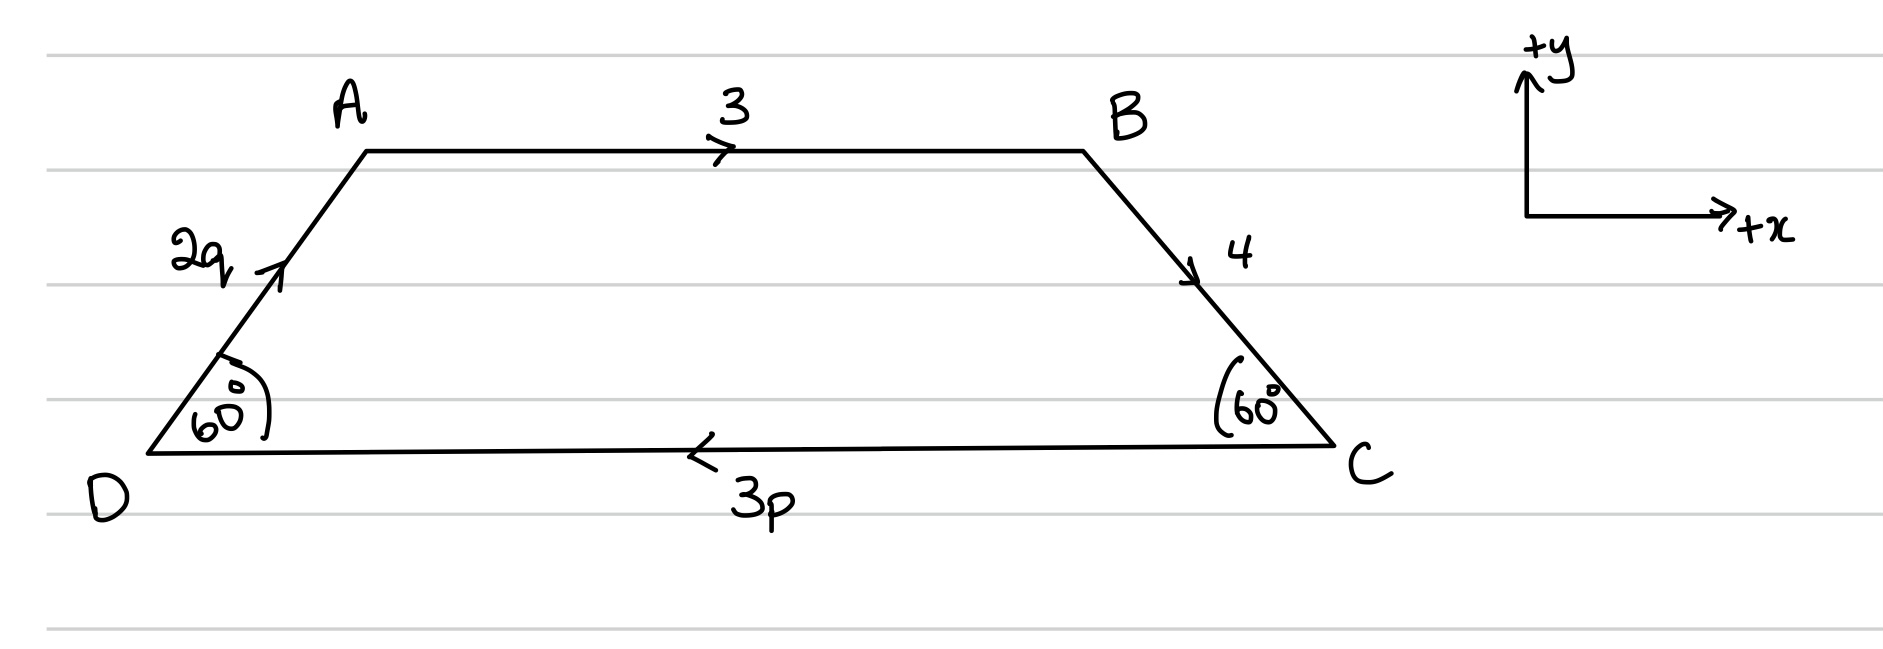
\includegraphics[scale=0.25]{../2007/figures/2008Mq6Diagram2}
		\caption{\label{2008M:q6:Sketch2} Forces along ABCD.}
	\end{center}
\end{figure}




\textbf{\textit{Simplify and Diagram:}} \\ \\ 
\rfig{2008M:q6:Diagram2} shows all of the forces and angle measures on ABCD. We will assume that all the forces act on a single point particle.
\begin{figure}[H]
	\begin{center}
		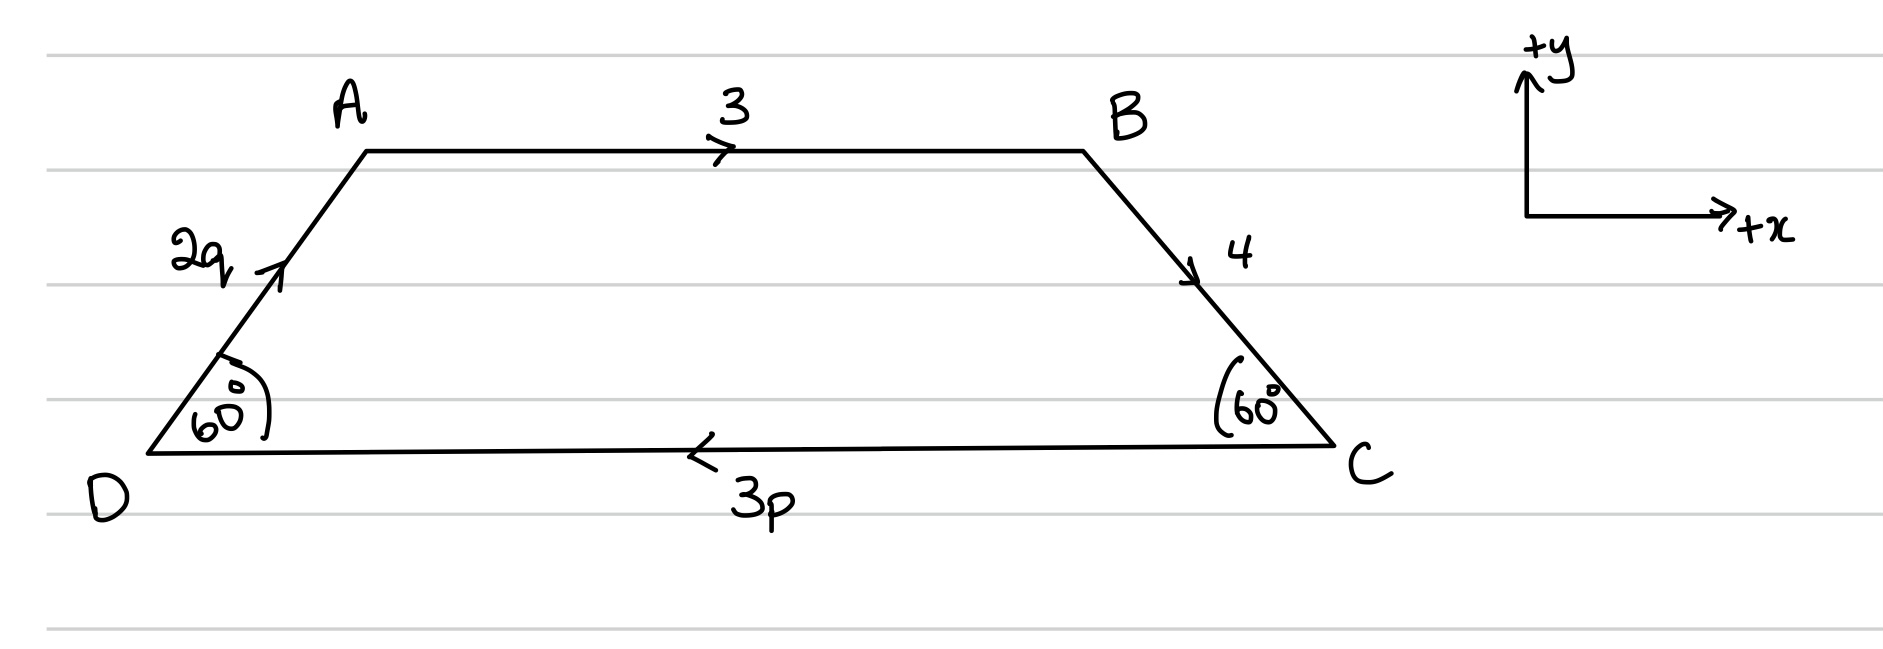
\includegraphics[scale=0.25]{../2007/figures/2008Mq6Diagram2}
		\caption{\label{2008M:q6:Diagram2} All forces and angles acting in ABCD.}
	\end{center}
\end{figure}

Let,
\begin{itemize}
	\item $\vec{AB}$ be the force acting from A to B.
	\item $\vec{BC}$ be the force acting from B to C.
	\item $\vec{CD}$ be the force acting from C to D.
	\item $\vec{DA}$ be the force acting from D to A.
\end{itemize}

As the system is in equilibrium, from Newton's Second Law, the resultant force on system must be 0. By resolving the forces in the $x$ and $y$ directions, we can solve for $p$ and $q$.




\textbf{\textit{Represent Mathematically:}} \\ \\
Resolving $\vec{AB}$, we get,
\begin{align}
	\vec{AB} & = |\vec{AB}|\xhat \nn \\
	         & = 3\xhat \,.
\end{align}

Resolving $\vec{BC}$, we get,
\begin{align}
	\vec{BC} & = |\vec{BC}|\cos(60)\xhat - |\vec{BC}|\sin(60)\yhat \nn \\
	         & = \left(4\times \frac{1}{2}\right)\xhat - \left(4\times \frac{\sqrt{3}}{2}\right)\yhat \nn \\
	         & = 2 \xhat - 2\sqrt{3}\yhat \,.
\end{align}

Resolving $\vec{CD}$, we get,
\begin{align}
	\vec{CD} & = -|\vec{CD}|\xhat \nn \\
			 & = -3p\xhat \,.
\end{align}

Resolving $\vec{DA}$, we get,
\begin{align}
	\vec{DA} & = |\vec{DA}|\cos(60)\xhat + |\vec{DA}|\sin(60)\yhat \nn \\
	         & = \left(2q\times \frac{1}{2}\right)\xhat + \left(2q\times\frac{\sqrt{3}}{2}\right)\yhat \nn \\
	         & = q\xhat + q\sqrt{3}\yhat \,.
\end{align}

As the system is in equilibrium, by Newton's 2nd Law, we get that,
\begin{align}
	\sum F_x & = 0 \nn \\
	\text{and} \nn \\
	\sum F_y & = 0 \,.
\end{align}




\textbf{\textit{Solve and Evaluate:}} \\ \\
Considering the $y$ direction, we get that,
\begin{align}
	\sum\vec{F}\yhat = 0\yhat & = -2\sqrt{3}\yhat + q\sqrt{3}\yhat \nn \\
	                   0\yhat & = (-2\sqrt{3} +q\sqrt{3})\yhat \nn \\
	        \implies   0 & =  (-2\sqrt{3} +q\sqrt{3}) \nn \\
					q\sqrt{3} & = 2\sqrt{3} \nn \\
				   \implies q & = 2 \,.
\end{align}

Considering the $x$ direction, we get that,
\begin{align}
	\sum\vec{F}\xhat = 0\xhat & = 3\xhat + 2\xhat -3p\xhat +q\xhat \nn \\
	                   0\xhat & = (3+2-3p+q)\xhat \nn \\
	\implies 0 & = 3+2-3p+q \nn \\
			 3p-q & = 5 \nn \\
	           3p & = 5+q \nn \\
	            p & = \frac{5+q}{3} \nn \\
	              & = \frac{5+2}{3} \nn \\
	              & = \frac{7}{3} \,.
\end{align}


\end{subquestions}